\section{RC Week 11}
\subsection{Generics, polymorphism and templated containers}
\begin{frame}{Preliminary: A container of pointer}
As a kind reminder we briefly discuss containers of pointers here. The key idea in the whole discussion again is the problem of the ownership. 

One must be crystal clear that a container of pointer actually owns the object, which means:

\begin{itemize}
	\item Pass to a container only things you have ownership. 
	\item When you pop from a container, you must take over ownership. 
	\item When an object has been passed to the container, it's the container's responsibility and authority to treat the object. You should not use the object in any way since you no longer owns the object.
\end{itemize}

With this in mind we take a look a few slides:

\end{frame}

\begin{frame}
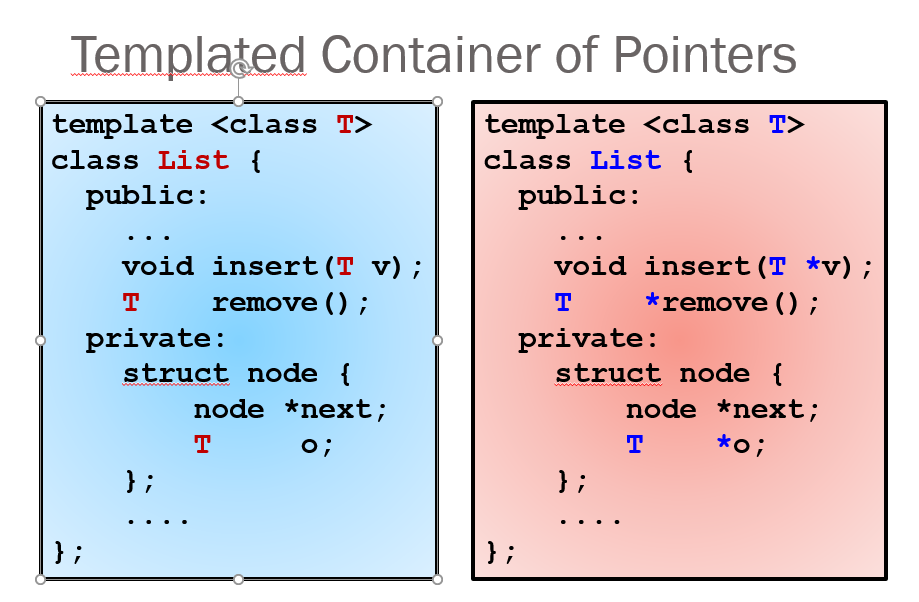
\includegraphics[scale=0.47]{fig/s1}
\end{frame}

\begin{frame}
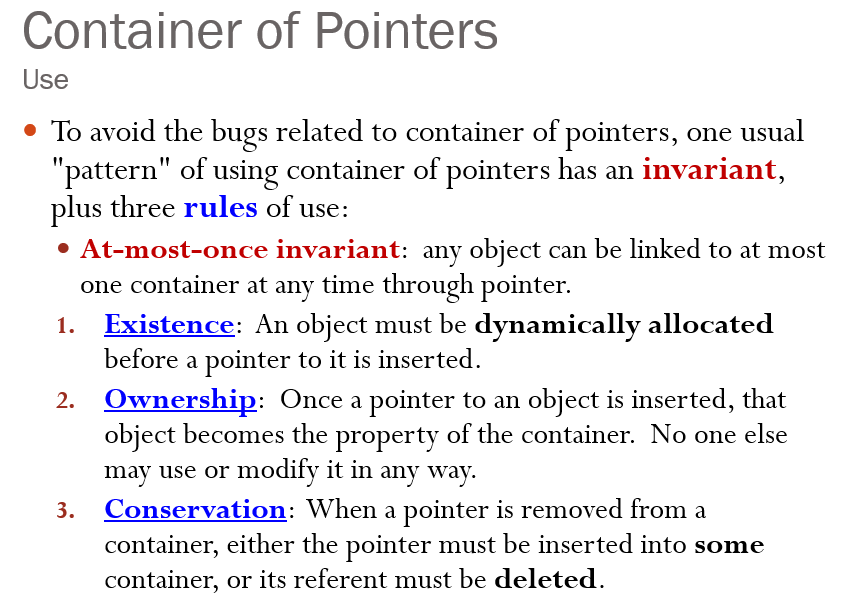
\includegraphics[scale=0.47]{fig/s2}
\end{frame}

\begin{frame}{Do not repeat your self}
Containers are objects to contain other objects, they do not have an intrinsic meaning. From now on we focus on \alert{Containter of pointers} (though we use a container of value in this example). Consider the example of a container of \texttt{char} and \texttt{int}:

\vspace{-0.1in}
\begin{figure}
	\centering
	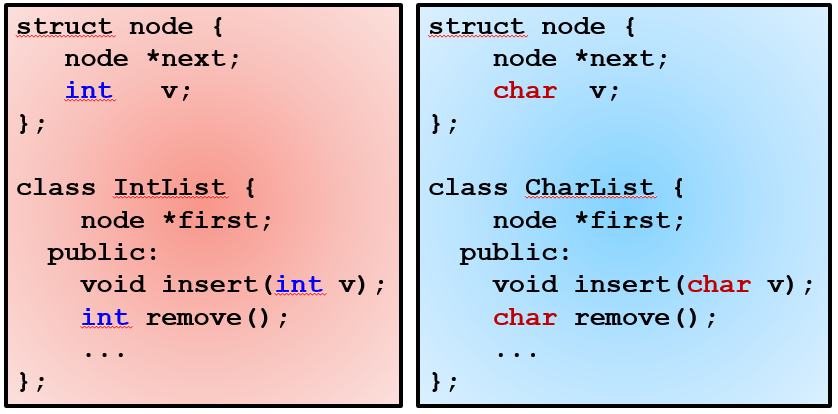
\includegraphics[scale=0.47]{fig/rc11dry}
\end{figure}

\end{frame}

\begin{frame}{Generics and polymorphism}
We would imagine they share the same implementation. Now our DRY principal suggest we should find a way to abstract out the almost identical implementation. 

Now we must familiar ourself to two widely used terms:

\begin{description}[Polymorphism]
	\item[Generics] A generic algorithm is an algorithm that does not depend on a specific type. Type can be specified later.
	\item[Polymorphism] Polymorphism is a property of code. A piece of code is said to be polymorphic, if it works on ``a range of" types. 
\end{description}

Clearly polymorphism is a technique to achieve generics. What we need to implement here is a generic algorithm (data structure), and we are going to use polymorphic code to achieve our purpose.
\end{frame}

\begin{frame}{Polymorphism tool box}
We first start by examining our polymorphism toolbox. In general there are 3 ways achieve (different levels) of polymorphism. 

Polymorphic code always involve a time where the ``real" implementation starts to step in. In general there are two timings:
\begin{description}[Compile-time]
	\item[Compile-time] The compiler ``injects" the real implementation into our polymorphic code when it is being compile. Sometimes called \textit{static polymorphism}.
	\item[Runtime] The polymorphic behavior is determined when it is needed at runtime. A typical example is \texttt{virtual} functions. It introduces overhead.
\end{description}

We now examine our choices:

\begin{description}[Overloading]
	\item[Overloading] Function / operator overloading. Limited power.
	\item[Subtyping] Virtual functions. Polymorphism through dynamic dispatch. This is runtime polymorphism.
	\item[Parametric] Templates in C++. Type as a parameter. 
\end{description}
\end{frame}

\begin{frame}[fragile]{Polymorphic containers}
Both of the second and third solution can be used to solve our problem at hand. We first look at the second one.  We now introduces \texttt{Polymorphic containers}. 

In a polymorphic container, the basic idea is to create a universal super type. Every type it it's subtype. And a container is written in terms of the universal super type.

The universal super type looks like the following:

\begin{minted}{c++}
struct Object {
	virtual ~Object() {}
	virtual Object* clone() = 0;
}
\end{minted}
 
Every class to be pushed into the container should be a subtype of this class. There are two questions: why are both methods virtual? Why do we need the \texttt{clone()} method.
\end{frame}

\begin{frame}{Polymorphic containers}
Note when we copy construct the constructor we also use copy copy constructor to copy the contained objects. 

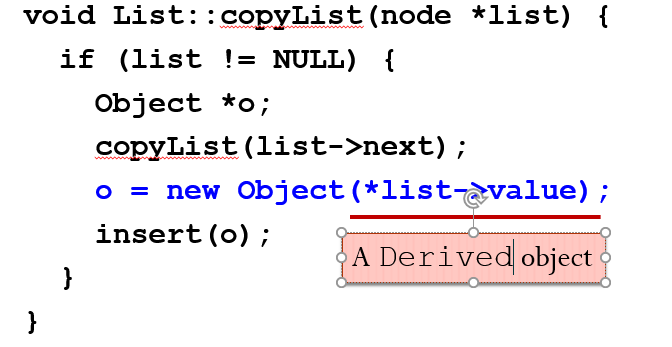
\includegraphics[scale=0.4]{fig/rc11pc1}

But unfortunately this simply cannot work. Remember that constructors cannot be virtual, since it is not possible for a base class object to setup invariants for a derived class object. 

Note above code does compile (why?). However what we get from such construction is an empty, useless \texttt{Object} class instance.
\end{frame}

\begin{frame}[fragile]{Polymorphic containers: copying}
\small
The solution is to ask the derived class instance to make a copy itself. This gives us the \texttt{clone()} method in the previous slides. This methods asks the object to make a copy of itself and returns a ptr to base class.  

Now our copy method can be written as follows:

\begin{minted}{c++}
void List::copyList(node *list){
    if (list != NULL) {
        Object *o; copyList(list->next);
        o = list->value->clone(); insert(o); } }
\end{minted}

Note this design makes sense from an interface point of view. In order for an object to be put inside a container it must be copyable. For normal container this is checked by the compile for the copy constructor (since the compiler knows the type in question). For polymorphic container since the compiler do not know what type is contained in advance so we must specify the constraint by ourself, namely through adding a \texttt{clone()} method.
\end{frame}

\begin{frame}[fragile]{Type Erasure}
We would like to make a final note. Consider when you pop something out of the container. The container only knows that the value is of type \texttt{Object*}. But you know it is actually an instance of \texttt{Derived*}. And most likely you need to use it as a \texttt{Derived} object. You need to transform a base class pointer to a derived class pointer.

\vspace{0.1in}

This way you will need a cast:
\begin{minted}{c++}
Derived* bp = dynamic_cast<Derived *>(list.remove());
\end{minted} 
The \texttt{dynamic\_cast<>} checks at \alert{runtime} if the pointer of base class is actually a pointer of derived class. If not so it returns \texttt{nullptr}. 
\end{frame}

\begin{frame}{Type Erasure}
Note all this must happen at run-time. No checks will be done at compile time. This has both up-side and down-side:
\begin{itemize}
	\item Since actual type is involved only when used this allows for heterogeneous containers. The contained object does not have to of the same type. This is a huge gain.
	\item However the cost is also significant! Since all checks are done at runtime, there is not type check at compile time either. Type mismatch will be deferred to runtime. This makes writing type safe code much harder!
\end{itemize}
Since essentially we are ``erasing" the actual type information of the objects when we put them into the container, this strategy is often called \textit{type erasure}. 

Problematic as it seems, \texttt{JAVA} choses to use type erasure when it comes to generics. This is one of the debatable feature of the language. 
\end{frame}

\begin{frame}{Poor man's template C++}
Now we turn to \texttt{template}, which is so called \textit{parametric polymorphism}. Before we introduce that in C++, I would like to familiarize you with a piece of code in C++:
\inputminted[]{c++}{code/rc11cp/poly.cpp}
\end{frame}

\begin{frame}[fragile]{Poor man's template in C++}
The code seems very cryptic at first. We now look at what it does by expanding the macros. \texttt{SWAP(int)} would be expanded into \texttt{swap\_int}. The two sharp signs means concatenating. An \texttt{SWAP\_IMPL(swap)} will be expanded into.
\begin{minted}{c++}
static void swap_int (int &x, int &y) {
    int t = x; x = y; y = x; 
}
\end{minted}
This is a very straight forward swapping two integers. As you can see this way we can reuse the \texttt{swap} function easily for different types by simpling use \texttt{SWAP\_IMPL} to create an implementation for different types and call them with \texttt{SWAP()}. 

Further more we can put the two macro definitions into a header file and include the when we need to. 
\end{frame}

\begin{frame}{Templates}
A template in C++ does exactly the same (for now. It if far more complicated if you explore deeper). When you write a template, for example:
\begin{columns}
	\column[]{.4\textwidth}
	
	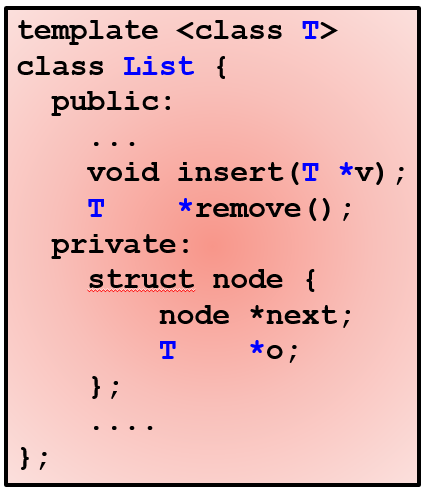
\includegraphics[scale=0.4]{fig/rc11pc3}
		
	\column[]{.6\textwidth}
	\vspace{-.3in}
	\begin{itemize}
		\small
		\item \texttt{T} is called a template parameter. It is usually a \texttt{class}, but it can be a value (e.g. an \texttt{int}). 
		\item The traditional way of specifying the type parameter is through \texttt{template<class T>}. But after C++11 one could use \texttt{template<typename T>}. 
		\item A template is much like a macro. When it comes to using it, the compiler uses an actual type to replace the type argument, and generate a version of implement for that type.
	\end{itemize}
\end{columns}
\end{frame}

\begin{frame}[fragile]{Template instantiation}
When you use a templated class, for example:
\begin{minted}{c++}
List<int> intList;
\end{minted}
The compiler will automatically produce a version of the actual code with the \texttt{int} as the parameter. This process is called \textit{template instantiation}. Template instantiation is conceptually the compiler writing \texttt{SWAP\_IMPL(int)} for us. 

We would like to make a footnote here. A template is by no means a type. A template is not a type since you cannot have a variable of \texttt{List} type clearly. It can be \texttt{List<int>} or \texttt{List<double>}, but simply is not \texttt{List}. A template is incomplete. It becomes a type when you put an actual type argument into it. 

In some literature templates are refered as a \textit{dependent type}.
You should notice this behavior is very much like a \textit{function}, which takes in a type and spits out another type. This function is ``sort of" evaluated in \alert{compile type}. 
\end{frame}

\begin{frame}[fragile]{A comment on the syntax}
Templates and \alert{their implementation} is almost always written in a header file (I would say always if not for the project). Libraries consists only of template classes are often called header libraries. The reason behind this should be simple from the previous poor-man's template example. 

There are in general two ways of implementing a templated class method. 
\begin{itemize}
	\item You can implement it inside the declaration.
	\item You can implement separately. 
\end{itemize}
For the second method:
\begin{minted}{c++}
template <class T> void List<T>::isEmpty() {...}
\end{minted}
\alert{The beginning \texttt{templated <class T>} must be there}. Note the method is implemented \alert{within the namespace \texttt{List<T>}}. This makes sense since namespaces corresponds to types, and \texttt{List<T>} is a type, \texttt{List} is not. 
\end{frame}

\begin{frame}[fragile]{A comment on the syntax}
We would like to make a comment on the following slide (ch21,30):
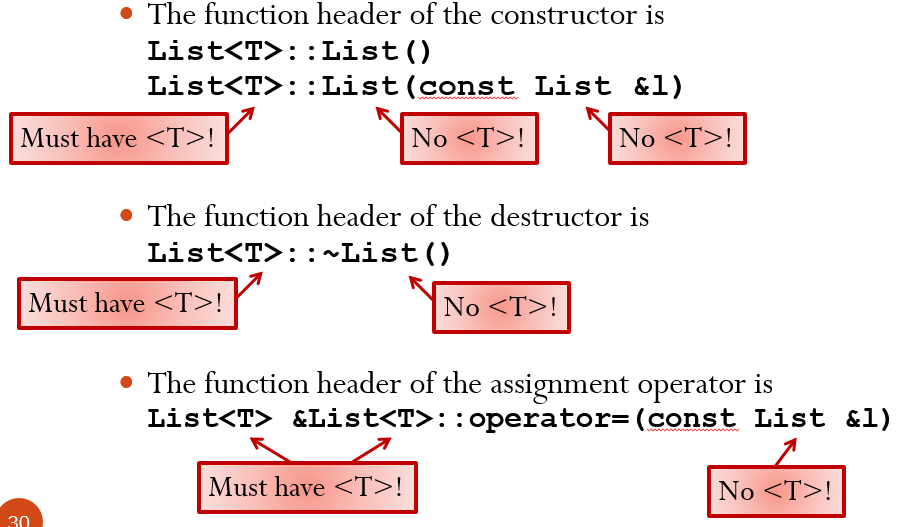
\includegraphics[scale=0.4]{fig/rc11p4}
\end{frame}

\begin{frame}[fragile]{A comment on the syntax}
We would like to make a comment on the following slide (ch21,30):

\vspace{0.1in}
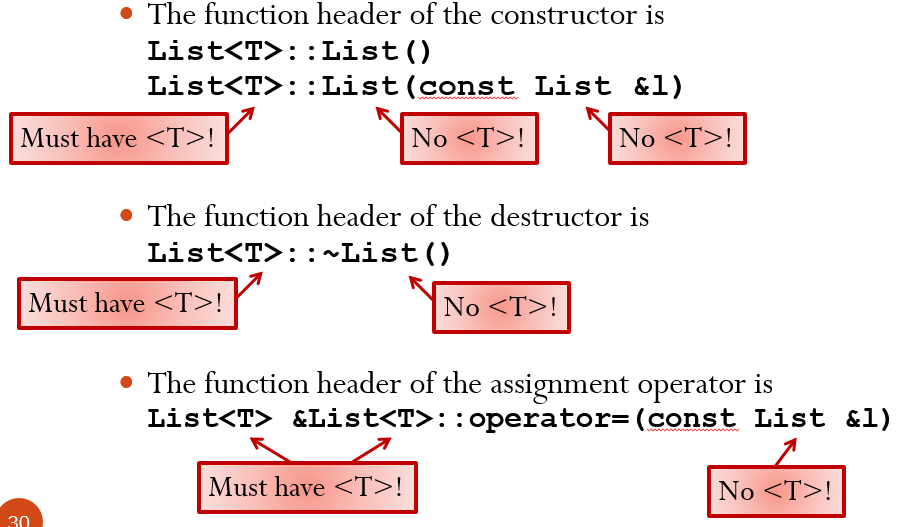
\includegraphics[scale=0.4]{fig/rc11p4}
\end{frame}

\begin{frame}[fragile]{A comment on the syntax}
You should find this to be very weired. Take a look at 
\begin{minted}{c++}
List<T>& List<T>::operator=(const List &l);
\end{minted}
Now what is the type of \texttt{l}? We have commented that \texttt{List} does not name a type. But clearly \texttt{l} is function argument and it must have a type. The professor commented ``No \texttt{<T>}!".

After a little research this is called a injected-class-name. Basically if you write \texttt{List} is a templated class, it will be inferred as \texttt{List<T>}, so we could use \texttt{List} as a shorthand of \texttt{List<T>} inside class declaration. We would like to note:
\begin{itemize}
	\item It is syntactically correct to write \texttt{List<T>}.
	\item It is also the recommended way as long as it does not impact readability too much, since it enhances clarity and makes more sense.
\end{itemize}
\alert{Note the name of the ctor/dtor must be \texttt{List}, not \texttt{List<T>}}.
\end{frame}

\begin{frame}[fragile]{A comment on the syntax}
We would like to emphasize on one thing, consider the following code
\begin{minted}{c++}
// Create a static list of integers
List<int> li;
// Create a dynamic list of integers
List<int> *lip = new List<int>;
// Create a dynamic list of doubles.
List<double> *ldp = new List<double>;
\end{minted}
Essentially forms \texttt{List<int>} are no difference to a regular \texttt{int}, \texttt{IntSet} etc. Anywhere a type can be use, such form can be use. For example it is possible to inherit from a templated type:
\begin{minted}{c++}
class Foo : public: List<int> {...}
\end{minted}
And then override some of its methods. 
\end{frame}

\begin{frame}{Compile time polymorphism trade-offs}
\small
Now we are at the core of compile time polymorphism. Templates are instantiated at compile time. The instantiation process is essentially the compiler deciding when to plug in the actual implementation. This gives us the following trade-offs:
\begin{itemize}
	\item It enhance code safety, by a lot. After substituting the type parameter with the actual type the compiler will be able to perform type checks. Type mismatches will be caught so that code correctness is improved.
	\item It improves performance (compared to polymorphic containers). Since the dispatch is done at compile time there is no run-time overhead. Compile-time dispatch also allows for further (much more) optimizations.
\end{itemize}

Above two are the major reasons people use templates. This is also why standard libraries choose to use templates to implement generic containers, since C++ is a language that focuses on performance and static typing. 
\end{frame}

\begin{frame}{Compile time polymorphism trade-offs}
\small
Now we take a look at the down sides
\begin{itemize}
	\item It prolongs compile time (a lot). The template system of C++ is so powerful that it self is Turing complete: meaning it is possible to write algorithms in terms of templates, or infinite loops that crashes the compiler.
	\item It increases the executable size. Each template instantiation creates more code. This gets worse combined with the C++'s ``one file per object" rule, as we will see next.
\end{itemize}

The first point is not really a pure down side. Some people heavily exploit the first point and ends up creating a whole new area of programming, called \textit{meta-programming}. 

The second down side is generally OK for most desktop applications since people have large memories. But for embedded applications where memories are scares, this basically rules STLs out from the embedded use. 

Another problem with templates is it complicates the compiler by a lot. However it is not a bad news for you.
\end{frame}

\begin{frame}[fragile]{Operator overloading} 
We now fill in the final piece of puzzle, i.e. operator overloading. We have introduced this in the previous slides. See page 253/254. 

Again just as a reminder there are two ways to write an overloaded operator:
\begin{itemize}
	\item As a class method of the first operand (if there are multiple operands)
	\item Write as a normal method.
\end{itemize}

The second approach is very common for overloading the extraction / push operator on a I/O stream (pay attention to the return type of the function).  For example:

\begin{minted}{c++}
ostream& operator<< (ostream &s, const MyClass &r) {...}
\end{minted}

allows you to print to \texttt{cout} and \texttt{fstream} (why?) by:
\begin{minted}{c++}
Ofstream file(...); MyClass obj(...);
file << obj; cout << obj;
\end{minted} 

\end{frame}

\begin{frame}[fragile]{\texttt{friend} keyword}
\small
In our previous example \texttt{operator<<} might need to access private member of \texttt{MyClass} instance. You could provide an accessing operator for each of the member, but often it is not a good idea (why?). 

One workaround is specifically grant \texttt{operator<<(ostream \&s, const MyClass \&r)} access to the protected members. This can be done by using the \texttt{friend} keyword:

\begin{minted}{c++}
class MyClass {
    friend ostream& operator<< (ostream &s, const MyClass &r);}
\end{minted}

It doesn't matter where this is marked \texttt{public} or \texttt{private}. Note \texttt{friend} can also grant access to regular functions and even classes:

\begin{minted}{c++}
class MyClass { 
    friend class Bar; friend int foo(double foo);}
\end{minted}

Pay attention that \texttt{friend} is not mutual. If \texttt{ClassA} declares \texttt{ClassB} as \texttt{friend}. \texttt{ClassB} can access \texttt{ClassA}'s private member, but the other way around doesn't work. 
\end{frame}